\documentclass[13pt, a4paper, oneside]{book}

%usepackage
\usepackage[]{amsthm, bm, color, framed, graphicx, hyperref, mathrsfs}
\usepackage{amssymb, amsmath, float}
\usepackage[most]{tcolorbox}
\usepackage{enumerate}

\setlength{\parindent}{0pt}
\definecolor{shadecolor}{RGB}{241, 241, 255}

% English theorem environment

\newtheorem{theorem}{Theorem}[section]
\newtheorem{lemma}[theorem]{Lemma}
\newtheorem{pro}[theorem]{Proposition}
\newtheorem{cor}[theorem]{Corollary}
% \newtheorem{definition}{Definition}[section]
\newtheorem{remark}{Remark}[section]
\newtheorem{example}{Example}[section]
\newtheorem*{Claim}{Claim}
\newtheorem*{Pre}{Preliminaries}
\newenvironment{Proof}{\begin{proof}[Proof]}{\end{proof}}
\newtcbtheorem[
number within = section % 按每个 section 分别编号
]{definition% 环境名
}{Definition% 这个参数可以设成“定理”“引理”“推论”等,编号就会变成“定理 1.1”“引理 1.1”“推论 1.1”等
}{
	attach title to upper = \par \vspace{1ex}, % 不要单独的标题栏,定理名完了之后分段,加上适量空白
	separator sign = \par, % 定理编号和定理名字之间用什么分隔;默认是冒号
	sharp corners, % 直角;默认是圆角
	enhanced jigsaw, frame hidden, % 隐藏 tcb 边框
	colback = shadecolor, % 背景色
	coltitle = black, % 标题(定理编号和名字)的颜色
	breakable
}{definition% label 前缀
}

%Basic Information

\title{\textbf{The Foundations of Algebra's Prequisite Course}}
\author{Shi Boyuan}
\date{\today}

\begin{document}
	%Introduction Area
	
	\maketitle
	\tableofcontents
	
	%body
	
	\chapter{The Foundations of Algebra} %代数学基础
	
	\section{The Prerequisite Course} %前置课程
	
	\begin{Pre}
		This Course is taught by Luosw and its purpose is to introduce basic concepts in fundations of algebra
	\end{Pre}
	
	What is mathematics? Bourbaki says: In mathematics we study \\
	\hspace*{0.3cm} Structures defined on sets \\
	\hspace*{0.3cm} Maps preserving structures \\
	
	\subsection{Classical set Theory}  %古典集合论
	
	Learning classical set theory can be divided into two parts \\
	\hspace*{0.3cm} The relation and operation between sets \\
	\hspace*{0.6cm} $\subseteq \quad \times \quad \sqcup \quad P\left( S \right) \enspace or \enspace 2^{S} \quad \cup \quad \cap$ \\
	\hspace*{0.3cm} The set-functions \\
	\hspace*{0.6cm} $ A \longleftrightarrow B \quad A \hookrightarrow B \quad A \twoheadrightarrow B $
	
	\subsubsection{Relations and Operations between sets}
	
	\begin{definition}{Direct Product}{}
		Direct Product $ \left( \times \right) $
	\end{definition}
	
	\begin{definition}{Disjoint union or coproduct}{}
		Disjoint union or coproduct $ \left( \sqcup \right) $
	\end{definition}
	
	\begin{remark}
		There are some relations between product and coproduct.An explanation will be given later.
	\end{remark}
	
	\begin{remark}
		if $A \cap B = \emptyset $,then $ A \cup B = A \sqcup B $
	\end{remark}
	
	\begin{definition}{Power Sets}{}
		Power Sets, $P(A)$ or $ 2^{A} $
	\end{definition}
	
	\begin{remark}
		$P(\mathbb{N})$is special.It's the first uncountable set discovered by our mankind
	\end{remark}

	\subsubsection{Mapping between Sets}  %集合间的映射
	
	\begin{definition}{Set-function}{}
		Set-functions, Def by $\mathbb{A} \times \mathbb{B}$,$f:A \rightarrow B$\\
	\end{definition}
	
	\begin{definition}{Image}{}
		Image
	\end{definition}
	
	\begin{definition}{Injection and surjection}{}
		Injection and surjection \\
		Injective $f: A \hookrightarrow B$ \\
		Surjective $ f: A \twoheadrightarrow B $
	\end{definition}
	
	\begin{definition}{Bijection or isomorphism}{}
		Bijection or isomorphism$~ f: A \leftrightarrow B $\\
	\end{definition}
	
	\begin{example}
		$ A \rightarrow {0} \times A $ is bijection,and $A \cong \left\{ 0 \right\} \times A$ \\
		$ \mathbb{A} \hookrightarrow \left\{ 0,1 \right\} \times \mathbb{A},a \longmapsto (0,a) $,which is a injection \\
		$$ A \underset{construct~a~isomorphism}{\overset{ \sim }{ \longrightarrow }} \left\{0\right\} \times A \overset{\iota}{\underset{inclusion}{\hookrightarrow}} \left\{0,1\right\} \times A $$
		so we find a decomposition of injection 
		
	\end{example}

	\subsubsection{Equivalence Relation}  %等价关系
	
	\begin{example}
		construct relation $<$ in $\mathbb{Z}$
	\end{example}
	
	\begin{definition}{Relation}{}
		Relation: A relation on a set $\mathbb{S}$ is defined by $\mathbb{R} \in \mathbb{S} \times \mathbb{S}$, If $(a,b) \in \mathbb{R}$,we say "a and b are related by $\mathbb{R}$" and we write aRb or $(a,b) \in \mathbb{R}$
	\end{definition}
	
	\begin{example}
		" $ = $ " in S: $ \{ (a,a) \mid a \in \mathbb{S} \} \subset \mathbb{S} \times \mathbb{S} $
	\end{example}
	
	\begin{definition}{Equivalence Relation}{}
		Equivalence Relation:If $\mathbb{R}$ is a relation on $\mathbb{S}$, satisfying \\
		1.(reflexivity) $aRa$ \\
		2.(symmetry) $aRb \Longrightarrow bRa$ \\
		3.(transitivity) $aRb,bRc \Longrightarrow aRc$
	\end{definition}
	
	\begin{remark}
		The definition's goal is to classify the set by the relation! 
	\end{remark}
	
	\begin{definition}{Equivalence Class}{}
		Equivalence Class, $ \left[ a \right]_{\sim} $
	\end{definition}

	Consider $ \left\{ \left[ a \right]_{\sim} \mid a \in \mathbb{S} \right\}$ as a Classification of sets
	
	\begin{definition}{Quotient Set}{}
		Quotient Set: $ S/ \sim = \left\{ \left[ a \right]_{\sim} \mid a \in \mathbb{S} \right\}$
	\end{definition}
	
	\begin{example}
		$ \mathbb{R} / = \cong \mathbb{R} $
	\end{example}
	
	\begin{example}
		Canonical Projection \\
		$\Pi$ : $ S \twoheadrightarrow S/ \sim $,$s \longmapsto \Pi (s) = \left[ s \right]_{\sim}$
	\end{example}
	
	\begin{example}
		$\mathbb{R}^2$,$\sim:x = x'$ \\
		$$ \mathbb{R}^2 \twoheadrightarrow \mathbb{R}^2/ \sim \overset{ \sim }{\longrightarrow} \mathbb{R}$$
		Appearently, $ \mathbb{R}^2 \underset{f}{ \twoheadrightarrow } \mathbb{R} $,Thus we find a dexcomposition of a surjection
	\end{example}
	
	\begin{example}
		we can use $\mathbb{Z} \times \mathbb{Z} \backslash \left\{0\right\}, (p,q) \sim (p',q') \Longleftrightarrow pq' = qp'$,$\left( \mathbb{Z} \times \mathbb{Z} \backslash \left\{0\right\} \right) / \sim$ to construct a isomorphism to $\mathbb{Q}$
	\end{example}
	
	\begin{pro}
		If $\mathbb{A} \overset{f}{\longrightarrow} \mathbb{B}$ is a set-function, we define a relation  $ \sim_{f} $ on $\mathbb{A}$ by $ a\sim_{f} b \overset{def}{\Longleftrightarrow} f(a) = f(b) $, then $\sim_{f}$ is an equivalence relation.
	\end{pro}
	
	\begin{proof}
		1.reflexivity:... \\
		2.symmetry:... \\
		3.transitivity:... 
	\end{proof}
	
	\begin{theorem}
		\Large \textbf{Canonical Decomposition} \\
		$$ \mathbb{A} \overset{projection}{\underset{\Pi}{\Longrightarrow}} \mathbb{A}/ \sim_{f} \overset{isomorphism}{\underset{\sim }{\longrightarrow}} Imf \underset{\iota}{\overset{inclusion}{\hookrightarrow}} \mathbb{B} \Longleftrightarrow \mathbb{A} \overset{f}{\longrightarrow} \mathbb{B}$$
	\end{theorem}
	
	\begin{remark}
		This conclusion is so fucking elegant!!! \\
		In group theory,$ A/kerf \cong imf $
	\end{remark}
	
	\begin{remark}
		product $\longleftrightarrow$ coproduct \\
		The product has a special property called universal property 
		\begin{figure}[h]
			\centering
			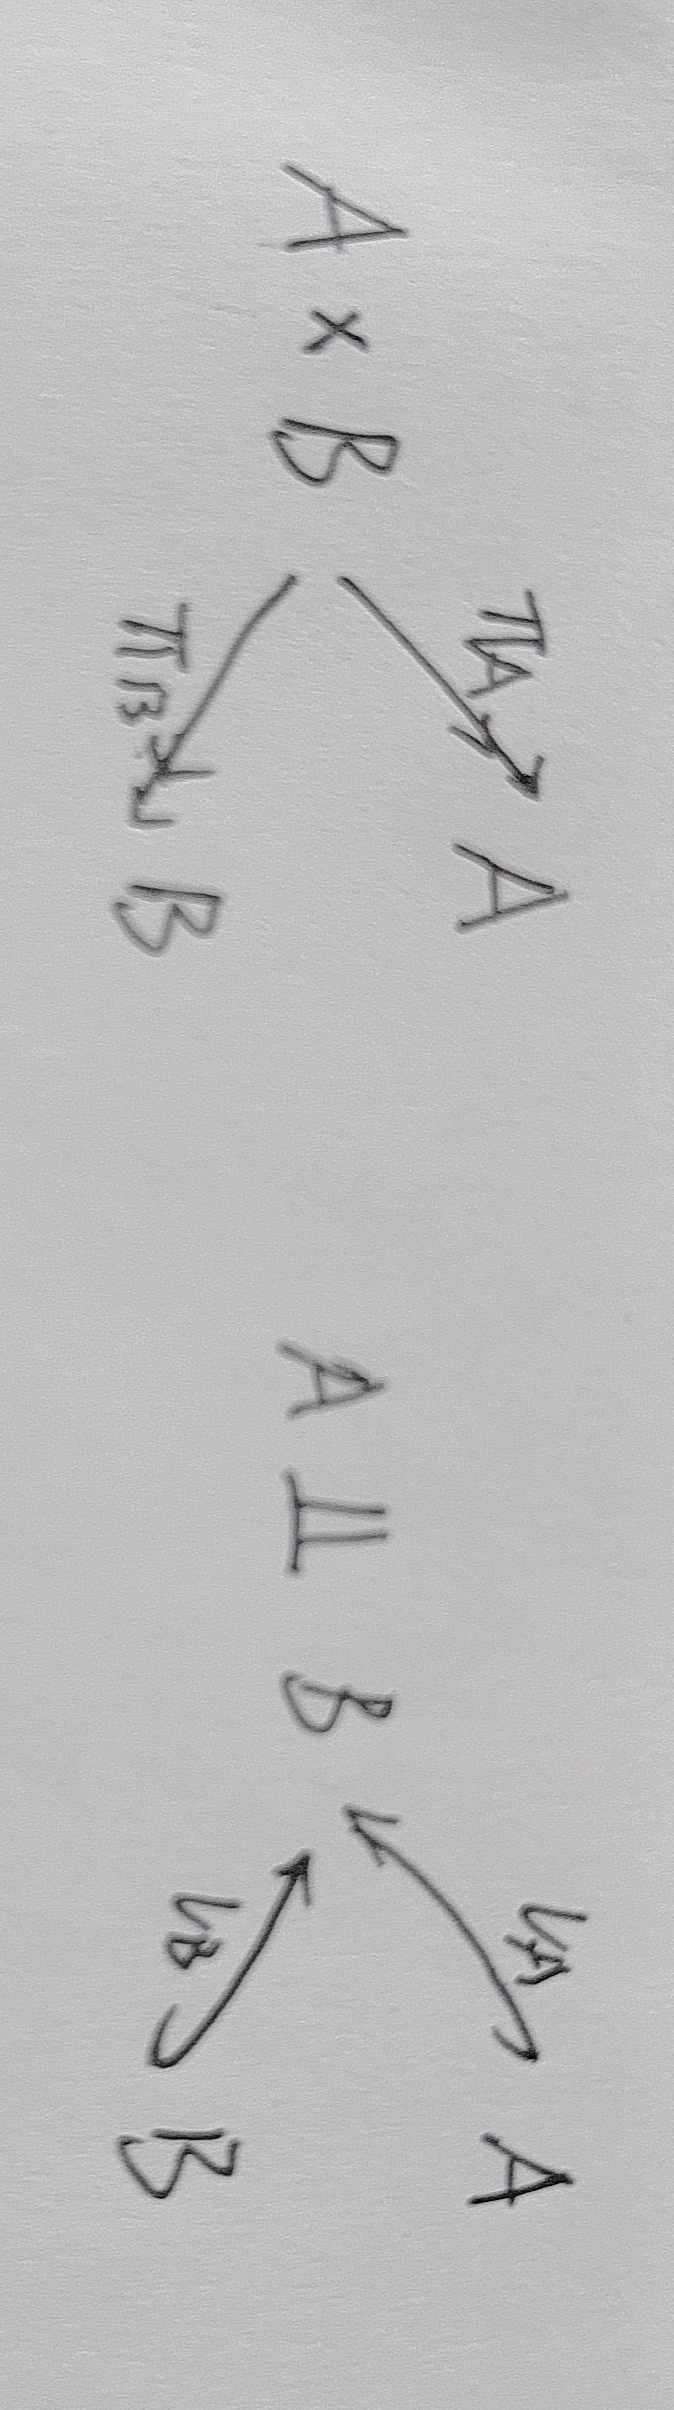
\includegraphics[width = 3cm, angle = 90]{Figures/F84C880A6B45B7D24D65345A7C341DFF.png}
		\end{figure} \\
		If there exists $\mathbb{C}$ and two set-functions $p:\mathbb{C} \longrightarrow \mathbb{A}$, $q: \mathbb{C} \longrightarrow \mathbb{B}$,then exists a \textbf{unique} $ \phi: \mathbb{C} \longrightarrow \mathbb{A} \times \mathbb{B} $,satisfying the diagram commutes 
		\begin{figure}[H]
			\centering
			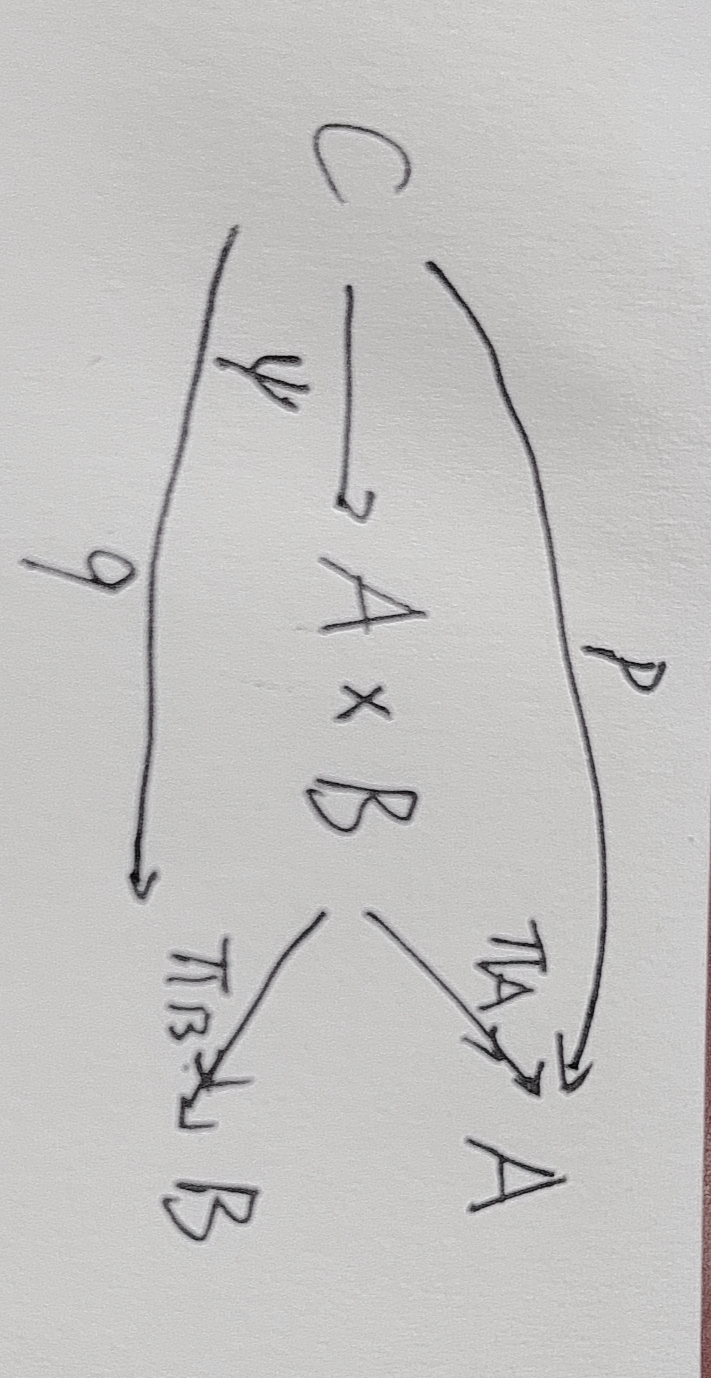
\includegraphics[width = 3cm, angle = 90]{Figures/72123EE8EFB9534DE4F4F5E6AB791CB7.png}
		\end{figure} 
		\begin{figure}[H]
			\centering
			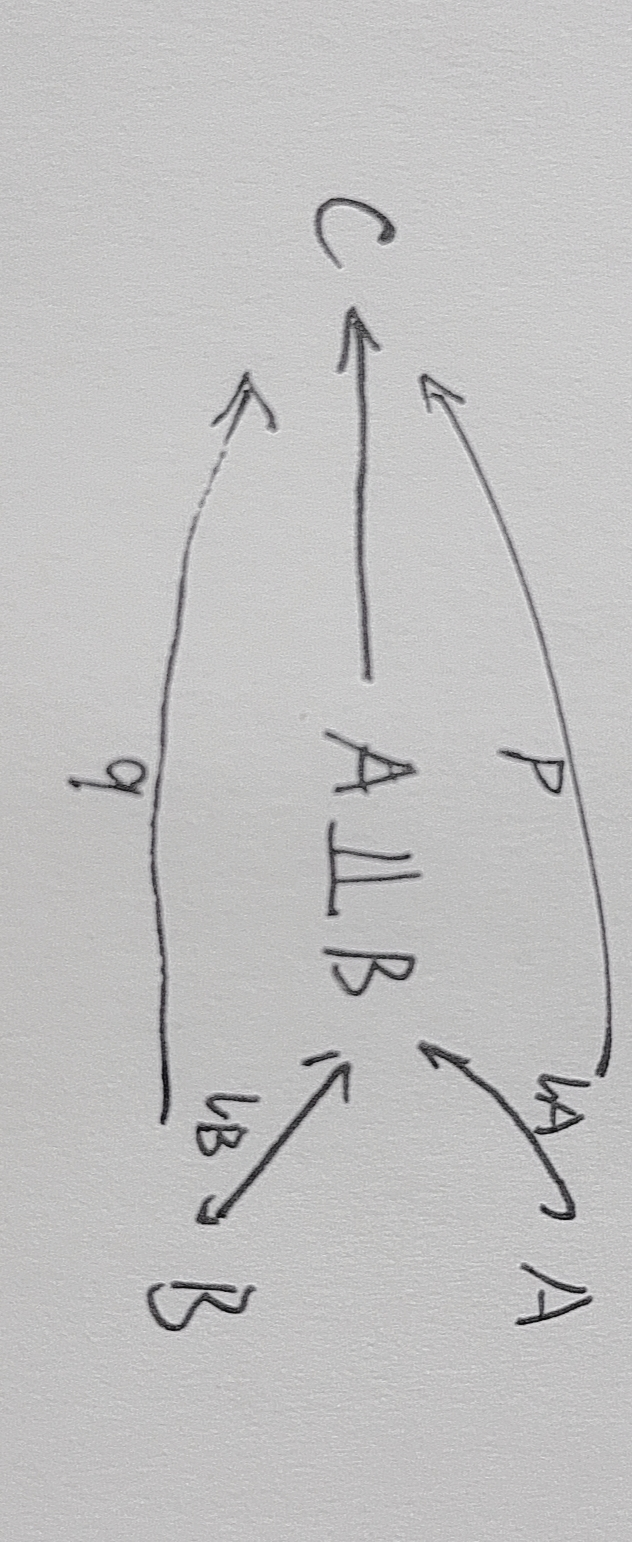
\includegraphics[width = 3cm,angle=90]{Figures/8DCAEE06D322292D4DA355344289906D.png}
		\end{figure}
		These pictures is a interpretation to the special property \\
	\end{remark}
	
	\newpage
	\subsection{Elementary Number Theory}  %初等数论
	
	This is the main content of this section. 
	\begin{figure}[H]
		\centering
		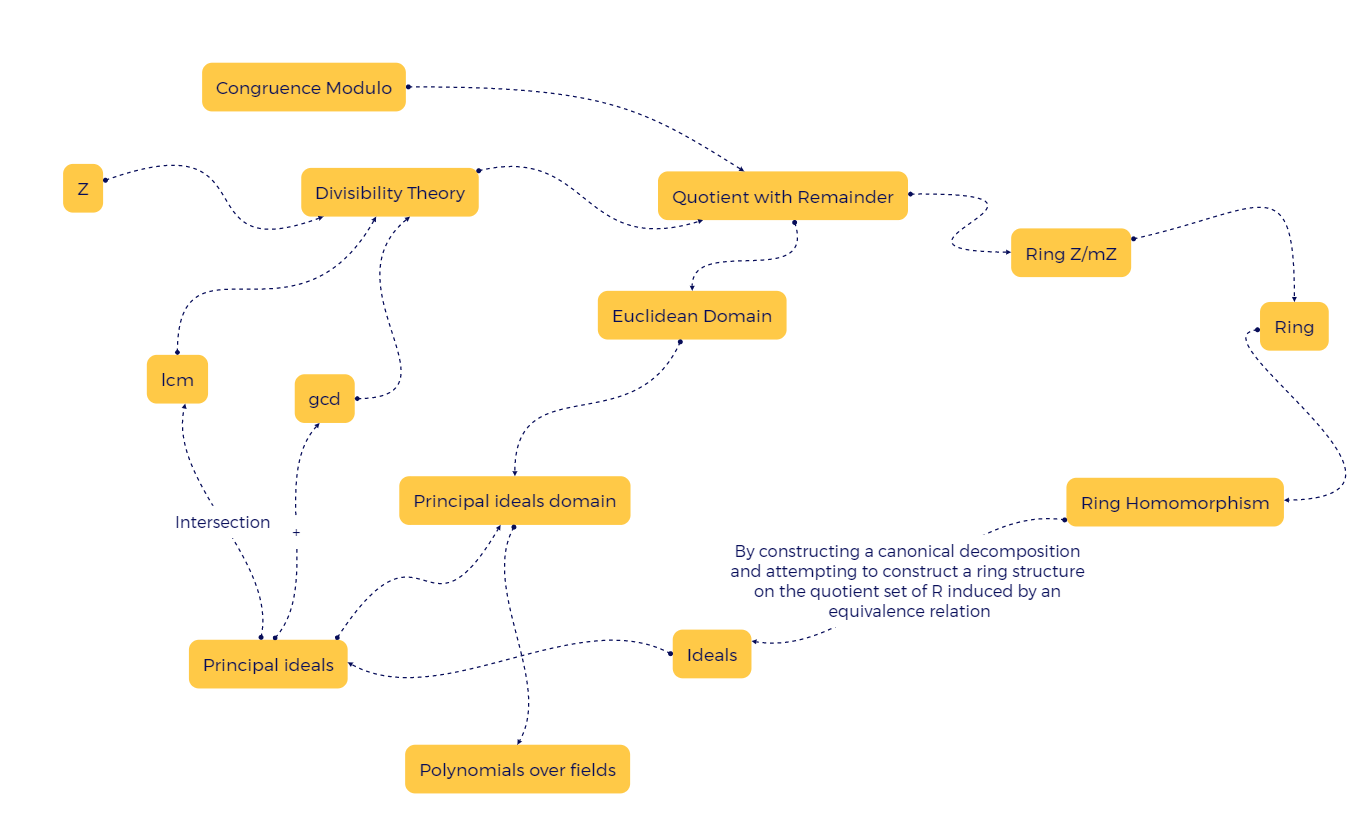
\includegraphics[width=15cm]{Figures/QQ20250920-154205.png}
	\end{figure}
	
	\subsubsection{Divisibility Theory}
	The Divisibility Theory is derived from the concept of division.
	
	\begin{definition}{Divisible}{}
		Divisible:$b \mid a$,and we say " a is divisible by b ",we call b is a divisor of a
	\end{definition}
	
	\begin{pro}
		There is some property, but I think it's not significant
	\end{pro}
	
	\begin{remark}
		$a \mid b, b \mid a \Longleftrightarrow \left| a \right| = \left| b \right|$
	\end{remark}
	If not divisible?
	
	\subsubsection{Quotient with Remainder}
	
	\begin{theorem}
		Let $a \in \mathbb{Z}, b \in \mathbb{Z} \backslash {0}$,then exists unique $(q,r) \in \mathbb{Z}^2$ satisfying $a = bq+r$ and $0 \leq r < \left|b\right|$
	\end{theorem}
	
	\begin{proof}
		I think it's easy
	\end{proof}
	
	\newpage
	\subsection{Ring}
	
	\subsubsection{Congruence Modulo}
	
	\begin{definition}{Congruence Modulo}{}
		Congruence Modulo	:$\equiv_{m}$
	\end{definition}
	Consider the quotient set of $\mathbb{Z}$ by $\equiv_{m}$,$$ \mathbb{Z}/ \equiv_{m} = \left\{ \left[0\right]_{\equiv_{m}}, \left[1\right]_{\equiv_{m}}, ... ,\left[m-1\right]_{\equiv_{m}} \right\} $$
	$$\mathbb{Z} = \bigsqcup^{m-1}_{i = 0} \left[i\right]_{\equiv_{m}} = \bigsqcup^{m-1}_{i = 0} \overline{i} $$
	what is addition and multiplication?,we can define it as a mapping f,$f: \mathbb{S} \times \mathbb{S} \mapsto \mathbb{S}$,and now we have the definition of these calculations, naturally we will put these calculations(additions and multiplications) on sets, we still need The Addition and Multiplication in $\mathbb{Z} $'s beautiful properties in new defined operations
	\begin{definition}{Ring}{}
		Ring:A set $\mathbb{R}$ with two calculations $+,\cdot$ satisfying: \\
		1.$(a+b)+c = a+(b+c)$ \\
		2.There exists $0_R$ \\
		3.There exists $-a$ \\
		4.$a+b = b+a$ \\
		5.$(a \cdot b) \cdot c = a \cdot (b \cdot c)$ \\
		6.There exists $1_R$ \\
		7.$(a+b) \cdot c = ac + bc$ and $ a \cdot (b+c) = ab+ac $ \\
		Then we call $(\mathbb{R},+,\cdot)$ is a ring \\
		If $\cdot$ satisfies: 8.$ab=ba$, then we call $(\mathbb{R},+,\cdot)$ is a commutative ring
	\end{definition}
	Because we define ring from the addition and multplication in $ \mathbb{Z} $, so we can easily know that $(\mathbb{Z}, +, \cdot)$ is a ring \\
	We can see that the calculation on the ring is the addition and multiplication inherited from the integer, so this can inspire us to define the calculation in $\mathbb{Z}/ m\mathbb{Z}$,which is very Apparent, and our result is as follows. \\
	
	\begin{definition}{The Operations on $\mathbb{Z}/ \equiv_{m} $}{}
		$$ \mathbb{Z}/ \equiv_{m} \times \mathbb{Z}/ \equiv_{m} \overset{+_{\mathbb{Z}/ \equiv_{m}}}{\longrightarrow} \mathbb{Z}/ \equiv_{m} $$
		$$ (\overline{a}, \overline{b}) \overset{+_{\mathbb{Z}/ \equiv_{m}}}{\mapsto} \overline{a +_{\mathbb{Z}} b} $$
		$$ \mathbb{Z}/ \equiv_{m} \times \mathbb{Z}/ \equiv_{m} \overset{\cdot_{\mathbb{Z}/ \equiv_{m}}}{\longrightarrow} \mathbb{Z}/ \equiv_{m} $$
		$$ (\overline{a}, \overline{b}) \overset{\cdot_{\mathbb{Z}/ \equiv_{m}}}{\mapsto} \overline{a \cdot_{\mathbb{Z}} b} $$
	\end{definition}
	This is the inheritance from $\mathbb{Z}$, so we can know that $(\mathbb{Z}/ \equiv_{m},+,\cdot)$ is a ring without proof 
	
	$$\mathbb{Z}/ \equiv_{m} \overset{+,\cdot}{\underset{Algebra~Structure}{\longrightarrow}} \mathbb{Z} / m\mathbb{Z} = \left\{ \overline{0}, \overline{1}, ... ,\overline{m-1} \right\}$$
	
	\begin{example}
		Table of addition/multiplication
	\end{example}
	
	\subsubsection{Ring Homomorphism}
	Ring Homomorphism is a mapping that don't change the operation on rings
	
	\begin{definition}{Ring Homomorphism}{}
		Ring Homomorphism:Keep Operation structures and $1_\mathbb{S}$
	\end{definition}
	
	we know the canonical decomposition in mapping between sets, but how will the cannonical decomposition be when we are talking in rings? \\
	$$ \mathbb{R}_1 \overset{\theta}{\longrightarrow} \mathbb{R}_2 \Longleftrightarrow \mathbb{R}_1 \underset{\Pi}{\twoheadrightarrow} \mathbb{R}_1 / \sim_{\theta} \overset{\sim}{\longrightarrow} im\theta \underset{\iota}{\longrightarrow} \mathbb{R}_2 $$
	The $\theta$ is a \textbf{ring homomorphism} \\
	we hope that every step of supra is a ring homomorphism, Firstly,if we want the $\Pi$ to be a ring homomorphism,we need $\mathbb{R}_1 /\sim_{\theta}$ to be a ring at least \\
	$$ \mathbb{R}_1 / \sim_\theta \overset{Algebra~Structure}{\underset{+, \cdot}{\longrightarrow}} Ring $$
	Like The Operations on $\mathbb{Z}/ \equiv_{m} $, we can use $\mathbb{R}_1$ to  define the $\mathbb{R}_1 / \sim_{\theta}$,definition are given as follows.
	
	\begin{definition}{The Operations on $\mathbb{R}_1 / \sim_{\theta}$}{}
		$$ \mathbb{R}_{\sim_{\theta}} \times \mathbb{R}_{\sim_{\theta}} \overset{+_{\mathbb{R}_{\sim_{\theta}}}}{\longrightarrow} \mathbb{R}_{\sim_{\theta}} $$
		$$ \left[ r_1 \right]_{\sim_{\theta}} +_{\mathbb{R}_1/ \sim_{\theta}} \left[r_2\right]_{\sim_{\theta}} = \left[r_1 +_{\mathbb{R}_1} r_2\right]_{\sim_{\theta}} $$
		$$ \mathbb{R}_{\sim_{\theta}} \times \mathbb{R}_{\sim_{\theta}} \overset{\cdot_{\mathbb{R}_{\sim_{\theta}}}}{\longrightarrow} \mathbb{R}_{\sim_{\theta}} $$
		$$ \left[ r_1 \right]_{\sim_{\theta}} \cdot_{\mathbb{R}_1/ \sim_{\theta}} \left[r_2\right]_{\sim_{\theta}} = \left[r_1 \cdot_{\mathbb{R}_1} r_2\right]_{\sim_{\theta}} $$
	\end{definition}
	
	\begin{remark}
		we need to prove that the results do not change with the change of the representative element we selected.How to prove it, by using the definition!
	\end{remark}
	
	\begin{remark}
		$$ a \sim_{\theta} b \Longleftrightarrow \theta ( a-b ) = 0_{\mathbb{R}_2} $$
	\end{remark}
	
	\begin{definition}{Kernel}{}
		Kernel: $ Ker(\theta) = \left\{ r_1 \in \mathbb{R}_1 \mid \theta (r_1) = 0 \right\}$
	\end{definition}
	
	\begin{pro}
		$ a \sim_{\theta} b \Longleftrightarrow a-b \in Ker(\theta) $
	\end{pro}
	
	\begin{remark}
		$$ \mathbb{R}_1 \longrightarrow \mathbb{R}_1 / \sim_{\theta} \overset{+,\cdot}{\underset{Algebra~Structure}{\longrightarrow}} \mathbb{R}_1/ Ker(\theta) $$
		we all know $ \mathbb{R}_1/ \sim_{\theta} $ is 	quotient set and $ \mathbb{R}_1 / Ker(\theta) $ is quotient ring \\
		$ \mathbb{I} \overset{?}{\underset{Find~Ring~Structure}{\longrightarrow}} \mathbb{R}/ \mathbb{I}  $ \\
		Firstly, we can define a equivalence relation $ a \sim_{I} b \overset{def}{\Longleftrightarrow} a-b \in \mathbb{I} $, so we can define a $ \left[..\right]_{\mathbb{I}} $, so that we can define $ \mathbb{R}/ \mathbb{I} $\\
		1.Reflexibility: $0 \in \mathbb{I}$ \\
		2.Reflexivity: $ a \in \mathbb{I} \Longrightarrow -a \in \mathbb{I} $ \\
		3.Transitivity: $ a,b \in \mathbb{I} \Longrightarrow a+b \in \mathbb{I} $ \\
		Under the above constraints,we can make $ \mathbb{R}/ \mathbb{I} $ a quotient set, but we still need to add some operations($ +, \cdot $) on it to make it a quotient ring,and this operation will stricter the constraints. Finally, we call $\mathbb{I}$ the $\mathbb{R}$'s ideal.
	\end{remark}
	
	\subsubsection{Ideal}
	
	\begin{definition}{The Operations on $\mathbb{R}/ \mathbb{I}$}{}
		$$ \left[ r_1 \right]_{\sim_{\mathbb{I}}} +_{\mathbb{R}/ \mathbb{I}} \left[ r_2 \right]_{\sim_{\mathbb{I}}} = \left[ r_1 +_{\mathbb{R}} r_2 \right]_{\sim_{\mathbb{I}}}$$
		$$ \left[ r_1 \right]_{\sim_{\mathbb{I}}} \cdot_{\mathbb{R}/ \mathbb{I}} \left[ r_2 \right]_{\sim_{\mathbb{I}}} = \left[ r_1 \cdot_{\mathbb{R}} r_2 \right]_{\sim_{\mathbb{I}}}$$
		Others, we need to prove the results do not change with the change of the representative element we selected
	\end{definition}
	
	\begin{Proof}
		we know$$ r_1 \sim_{I} r_1', r_2 \sim_{I} r_2' $$
		then proof$$ \left[r_1 +r_2\right]_{\sim_{I}} = \left[r_1' + r_2'\right]_{\sim_{I}} $$
		this is easy by the Transitivity \\
		The next $$ r_1'r_2' - r_1r_2 \in \mathbb{I} \Longrightarrow -r_2'(r_1 -r_1') -r_1(r_2-r_2') \in \mathbb{I}$$
		so we have a new constraint $$ \forall a \in \mathbb{I}, c \in \mathbb{R}, ca \in \mathbb{I} $$
	\end{Proof}
	
	\begin{definition}{Ideal}{}
		Ideal: we assume $\mathbb{R}$ is a commutative ring\\
		\textbf{I stuck here for about 3 minutes to think about why $\mathbb{R}$ is a commutative ring and finally I got the reason, This is because when we are deriving from $ r_1'r_2' - r_1r_2$, we use the commutative law} \\
		We call $ \mathbb{I} $ an ideal of $\mathbb{R}$ iff \\
		$$ \forall a,b,\in \mathbb{I}, a+b \in \mathbb{I} $$
		$$ \forall a \in \mathbb{I}, c \in \mathbb{R}, ca \in \mathbb{I} $$
		\textbf{I stuck here for about 5 minutes to think about how can we get a $-1$ from $\mathbb{R}$ and finally I get: we can pick the $1_{\mathbb{R}}$ to the $-1_{\mathbb{R}}$}
	\end{definition}
	
	\begin{example}
		1.$Ker(\theta) \subset \mathbb{R}_1 \Longrightarrow Ker(\theta)$ is an ideal of $\mathbb{R}_1$ \\
		2.$ \mathbb{R} \overset{\Pi}{\twoheadrightarrow} \mathbb{R}/ \mathbb{I} $,then $Ker\Pi = \mathbb{I}$ \\
		3.$Ideal \Longleftrightarrow Kernel$
	\end{example}
	
	\begin{example}
		Using $\mathbb{Z} / m\mathbb{Z}$ as a example \\
		$$ \mathbb{Z} \longrightarrow \mathbb{Z}/ \equiv_{m} \longrightarrow \mathbb{Z}/ m\mathbb{Z} $$
		In fact, $m\mathbb{Z}$ is an ideal of $\mathbb{Z}$ \\
		so $ r\mathbb{R} $ is an ideal of $\mathbb{R}$
	\end{example}
	
	\begin{definition}{Principle Ideal}{}
		Principle Ideal:$(r) = \left\{ r \cdot r' \mid r' \in \mathbb{R} \right\}$, we call $(r)$ the principle ideal generated by r
	\end{definition}
	
	\begin{pro}
		Any ideal $\mathbb{I} \subset \mathbb{Z}$ is principle,so $\mathbb{Z}$ is \textbf{principle ideal domain}(PID)
	\end{pro}
	
	Can we generate new ideals from given ideals ?
	
	\begin{pro}
		If $\mathbb{I}_1, \mathbb{I}_2\subset \mathbb{R}$ ideal,then \\
		$$ \mathbb{I}_1 \cap \mathbb{I}_2 , \mathbb{I}_1 +\mathbb{I}_2, \mathbb{I}_1 \cdot \mathbb{I}_2 =\left\{ a_1b_1+a_2b_2 + ... +a_nb_n \mid a_1 ... a_n \in \mathbb{I}_1, b_1 ... b_n \in \mathbb{I}_2 \right\} $$ is ideal 
	\end{pro}
	
	From this, we can easily construct a connection between ideal and number theory
	
	\begin{definition}{From ideal to number theory}{}
		Under $\mathbb{Z}$
		$$ (a) \subset (b) \longrightarrow b\mid a $$
		$$ (a) + (b) = (d) \longrightarrow d = gcd(a,b) $$
		$$ (a) \cap (b) = (l) \longrightarrow l = lcm(a,b) $$
	\end{definition}
	
	\begin{theorem}
		Bezout's theorem: \\
		Given $a,b \in \mathbb{Z}$,then there exists $s,t \in \mathbb{Z}$,such that $$ as+bt =gcd(a,b) $$
		If there exists $d' \mid a, d' \mid b$. satisfying $d' = as+bt \Longrightarrow d' = gcd(a,b)$
	\end{theorem}
\end{document}